
\chapter{Moduli of curves}
\label{CurvesModuli chapter}\label{CurvesModuliChapter}


In the preceding chapter, we described the \emph{Hilbert scheme}, a fine moduli space for curves in projective space. In
this chapter we will discuss the second moduli space central to the theory of algebraic curves: $M_g$, which parametrizes isomorphism classes of smooth projective curves of genus $g$. As we'll see, $M_g$ is not a fine moduli space, but it comes close.

To describe the situation,  we will start with the case of curves of genus 1, where everything can be made explicit.


\section{Curves of genus 1}\label{Curves of genus 1}

Let $C$ be a smooth curve of genus 1. Any invertible sheaf of degree 2 on $C$ can be written as
\index{moduli space!of genus 1 curves}%
\index{genus 1 curve!moduli space of}%
$\sO_C(2p)$, and defines
a morphism to $\PP^1$ with 4 distinct branch points. Since the automorphism group of $C$ is transitive,
these 4 points in $\PP^1$ are independent of the choice of $p$, and are well-defined
up to an automorphism of $\PP^1` `$.    As explained in Section~\ref{branched covers},  this means that every such curve $C$ can be realized as the completion of an affine curve
$$
y^2 = f(x)
$$
where $f$ is a quartic polynomial with distinct roots:
\vspace*{-2pt}
$$
f(x) = \prod_{i=1}^4 (x - \lambda_i).
$$
Thus we would like to define $M_1$ to be the set of 4-tuples of
distinct points $\{\lambda_{1}, \dots, \lambda_{4}\}$ of $\PP^1$
\index{PGL@$\PGL_2$}%
modulo the action of $\Aut \PP^1 =
\PGL_2
$.

As we will explain in the next sections, quotients by infinite groups can behave badly,
but in this case we can compute the quotient in a much simpler way:
There is a unique automorphism of $\PP^1$ carrying the three points $\lambda_1, \lambda_2,\lambda_3$ to the points $0, 1$ and $\infty \in \PP^1$ respectively, so that we can write $C$ as the zero locus of
$$
y^2 = x(x-1)(x-\lambda)
$$
for some complex number $\lambda  \in \PP^1 \setminus \{0,1,\infty\}$; we'll call this curve $C_\lambda$.
This expression is not unique, since if we reordered the original
four points $\lambda_i$, we might arrive at a different value of
$\lambda$; for example, if we exchanged 0 and $\infty$ and fixed 1,
$\lambda$ would be replaced by $1/\lambda$. Thus the
symmetric group
\index{symmetric group}%
$S_4$ acts on the set $\AA^1 \setminus \{0,1,\infty\}$
and one can show that the orbit of $\lambda$ under this action is
$$
\let\frac\mfrac
 \left\{ \lambda, 1-\lambda, \frac{1}{\lambda}, \frac{1}{1-\lambda}, \frac{\lambda-1}{\lambda}, \frac{\lambda}{\lambda - 1} \right\}.
$$
There are 6 points in the orbit rather than 24 because the
Klein 4-group
\index{Klein 4-group}%
$K = \ZZ/2\times \ZZ/2 \subset S_4$ of
fixed-point-free involutions
acts trivially, so what we really have is an action of $S_4/K \cong S_3$.

Since $S_3$ is finite and $\PP^1 \setminus \{0,1,\infty\}$ is a normal affine curve, the quotient space by the action is again a normal affine curve whose points are in one-to-one
correspondence with the orbits, and thus with the set of curves of genus~1.
By
L\"uroth's theorem
\index{L\"uroth's theorem}%
(Theorem~\ref{Lueroth}), the quotient is rational, meaning that the
field of rational functions on the quotient\emdash that is, the
subfield of $\CC(\lambda)$ invariant under the action of $S_3$\emdash
is of the form $\CC(j)$ for some rational function $j(\lambda)$ of
degree 6. Of course, there are many possible generators of the field
of rational functions on the quotient; one that works is
\begin{equation}\label{formula for j}
j(\lambda) \colonequals  256\frac{(\lambda^2-\lambda + 1)^3}{\lambda^2(\lambda-1)^2},
\tag{$*$}
\end{equation}
known as the
\emph{$j$-function}.
\index{j@$j$-function|defi}%
 As $\lambda$ varies in $\PP^1 \setminus \{0,1,\infty\}$,
the values of
$j(\lambda)$
range over all of
$\AA^1` `$.

Summarizing, we have proven:

\begin{theorem}
\hskip-3pt
The set of isomorphism classes of smooth projective curves of genus$@1$
\index{genus 1!classification of curves}%
is in bijection with the points of the affine line $M_1 \cong \AA^1``$.
The bijection maps the curve defined by $y^2 = x(x-1)(x-\lambda)$
to  $j(\lambda)\in \AA^1` `$.
\end{theorem}

\subsection*{$M_1$ is a coarse moduli space}

 As we will see in Exercises~\ref{not fine 1} and~\ref{not fine 2},
$M_1$ is not a fine moduli space, but it comes close in two senses.

\begin{proposition}\label{M1 is coarse}
To any family $\pi : \cC \to B$  of smooth projective curves of
genus~$1$ over a reduced base $B$ we can associate a natural morphism of
schemes $$\phi : B \to M_1$$ whose value at any point $b \in B$ is the
$j$-invariant of the corresponding fiber~$C_b$.
\end{proposition}

\begin{proof}
To start, we will work locally in $B$: for a given $b_0 \in B$, we
will choose a suitably small neighborhood $U$ of $b_0 \in B$ and
restrict ourselves to the preimage $\cC_U = \pi^{-1}(U)$. The first
thing to do is to express the curves $C_b$ in our family as
2-sheeted covers
\index{2-sheeted cover!of $\PP\sp1$}%
of $\PP^1` `$, which is to say we want to choose an invertible sheaf
on $\cC_U$ having degree 2 on each fiber $C_b$. Since we're working
locally in $B$,
we can find a section $\rho : U \to \cC_U$ of $\pi : \cC \to B$. If we let $D = \rho(U) \subset \cC_U$ be the image, then we can take our invertible sheaf to be $\cL \colonequals  \cO_{\cC_U}(2D)$.

Next, we use the following result, which is a special case of the theorem on cohomology and base change
(see  \cite[Appendix, Theorems B.5 and B.9]{3264} or
\cite[Theorem 12.11]{Hartshorne1977}.)

\begin{theorem}[cohomology and base change]
If $f: X\to Y$ is a morphism and $\sF$ is
\index{cohomology and base change}%
\index{base change}%
a coherent sheaf on $X$ such that $H^{1}(\sF|_{f^{-1}(y)})= 0$ for all $y\in Y$, then
$h^{0}(\sF|_{f^{-1}(y)})$ is a constant function of $y$, and
$f_{*}(\sF)$ is a vector bundle of this rank.\qed
\end{theorem}

This result implies that the direct image $\cE \colonequals  \pi_*(\cO_{\cC_U}(2D))$ is locally free of rank 2, and we get a morphism $\cC_U \to \PP(\cE)$ expressing each curve $C_b$ as a 2-sheeted cover of the corresponding fiber $\PP(\cE_b)$. Again, since we are working locally in $B$, we can trivialize the bundle $\cE$, so that we get a diagram
$$
\small
\xymatrix@C=15pt@R=25pt{
\cC_U  \ar[rr]\ar[dr] && U\times\PP^1 \ar[dl]\\
&U
}
\vspace*{3pt}
$$
Once more restricting to a smaller neighborhood $U$ if necessary, we can write the family $\cC_U \to U$ as the locus
\vspace*{-3pt}
$$
y^2 = \prod_1^4 (x - \lambda_i),
$$
where the $\lambda_i$ are regular functions on $U$. The $j$-function of the $\lambda_i$  yields a map $U \to M_1$; since the value of the $j$-function at a point is determined by the isomorphism type of the fiber over this point, these maps agree on overlaps to give  the desired morphism $B \to M_1$.
\end{proof}



\subsection*{The good news}

The second way in which
$M_1$ comes close to being a fine moduli space
is seen in the next result:

\begin{proposition}\label{families on pullbacks} Let $B$ be a reduced scheme.
\begin{enumerate}
\item If $j : B \to \AA^1$ is any regular function on $B$, then there
  exists a finite cover $\alpha : B' \to B$ such that $j \circ \alpha$
  is the $j$-function of a family of curves of genus $1$ on $B'$.
\item If $\pi : \cC \to B$ and $\eta : \cD \to B$ are two families of
  curves of genus~$1$ with the same associated $j$-function, then there
  exists a finite cover $\alpha : B' \to B$ and an isomorphism $\cC
  \times_B B' \cong \cD \times_B B'$ such that the diagram
$$
\small
\xymatrix@C=15pt@R=25pt{
\cC \times_B B'   \ar[rr]\ar[dr] &&\cD \times_B B' \ar[dl]\\
&B'
}
$$
commutes.
\end{enumerate}
\end{proposition}

\begin{proof} For the first of these assertions, let
$$
B' \colonequals  \bigl\{@(b, \lambda)
 \in B \times (\AA^1 \setminus \{0,1\}) \mid j(b) = j(\lambda)@\bigr\} ,
$$
where $j(\lambda)$ is as given by formula~\eqref{formula for j}
on page~\pageref{formula for j}.
We have already described a family of curves of genus 1 over the
\emph{$\lambda$-line}
\index{lambda@$\lambda$-line}%
$\AA^1 \setminus \{0,1\}$; the pullback to $B'$ is
the desired family.

For the second half, we want to do something similar. Specifically, we want to choose sections $\sigma : B \to \cC$ and $\tau: B \to \cD$ and take
$$
B' \colonequals  \bigl\{@(b, \phi) \mid b \in B, \; \phi : C_b
\ruto {\,\cong} D_b  \text{ and } \phi(\sigma(b)) = \tau(b)@\bigr\};
$$
as a set, $B'$ is the set of isomorphisms between corresponding fibers
in the two families.
By Corollary~\ref{finite automorphism genus 1}, $B'$ is a finite cover
of $B$ and when we pull back the two families to $B'$ we have a
tautological isomorphism
between them. The only issue is how to give $B'$ an appropriate scheme
structure, and for this we can use the Isom scheme described at the
\index{Isom}%
end of Section~\ref{maps between curves}.
\end{proof}

Thus, $M_1$ is not a fine moduli space for smooth curves of genus 1, but it is the next best thing: we don't get a bijection between families of curves of genus 1 over a given base $B$ and maps $j : B \to M_1$; but we do get a map from the former to the latter with ``finite kernel and cokernel''.

\subsection*{Compactifying $M_1$}

A natural question to ask is, if every value of $j \in \AA^1$
corresponds to an isomorphism class of curves $C_j$ of genus 1, what
happens to the curves $C_j$ as $j$ goes to $\infty$?
Equivalently, what happens to the curve~$C_\lambda$ given as the double cover
$$
y^2 = x(x-1)(x - \lambda)
$$
when
$\lambda$ approaches 0, 1 or $\infty$\emdash the other branch points
of the double cover? The~answer is
seen
from the equation: when two
branch points of a double cover of smooth curves
coalesce
the
limiting curve has a node (Figure~\ref{smooth to singular}). In~fact,
there is a unique isomorphism class of irreducible curves of
\index{arithmetic genus}%
arithmetic genus
~1 having a node; it's represented by the curve
defined by
$y^2=x^2(x-1)$.

\begin{figure}
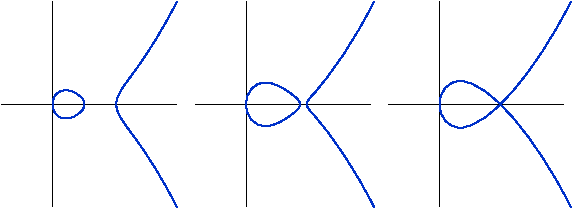
\includegraphics[width=3.6in]{main/cubic-la=0.5,0.9,1}
\centerline{\hfil
\footnotesize
\hbox to 1.15in{\hfil\hfil$\lambda=0.5$\hfil}\enspace
\hbox to 1.15in{\hfil\hfil$\lambda=0.9$\hfil}\enspace
\hbox to 1.15in{\hfil\hfil$\lambda=1$\hfil}\hfil
}
\caption{A curve of genus 1 degenerating to a rational curve with a node
in the family $y^2 = x(x-1)(x - \lambda)$.}
\label{smooth to singular}
\end{figure}


The upshot
is that if we enlarge the original class of curves parametrized by
$M_1$\emdash smooth projective curves of genus 1\emdash to the
slightly larger class
of
irreducible nodal projective curves of
arithmetic genus 1, we still have a coarse moduli space $\overkern31
M_1$ for this slightly larger class of objects. This enlarged moduli
space is obtained by adding one point ``at $\infty$'' to the existing
space $M_1 \cong \AA^1$ to form $\ovM_1 \cong \PP^1` `$.

This is an example of what is called a
\emph{modular compactification}.
\index{modular compactification}%
There is no precise definition, but if we have a
class of objects parametrized by a (noncompact) moduli space $M$ we
may be able enlarge the class of objects to be parametrized, with the
result that the moduli space $\ovM$ of the larger class is
compact.

Modular compactifications of a given moduli problem may or may not exist. It's sometimes a tricky problem to find a suitable class of objects to parametrize: if we don't add enough additional isomorphism classes, not every 1-parameter family of objects in our original class will have a limit in the larger class, meaning the enlarged moduli space will still not be compact; if we add too many,  1-parameter families may have more than one possible limit, meaning the enlarged space won't be separated. For example, in the family
 of curves $C_t$ given as
$$
C_t = V(y^2 -x^3 - t^2x - t^3)
,
$$
the $j$-function
is constant when $t\neq 0$, but  the limiting curve
$C_0$ has a
cusp
(Figure~\ref{smooth to cusp}). This shows that we could not have added
cuspidal curves to $M_1$.

\begin{figure}[b]
\def\quad{\hskip30pt}
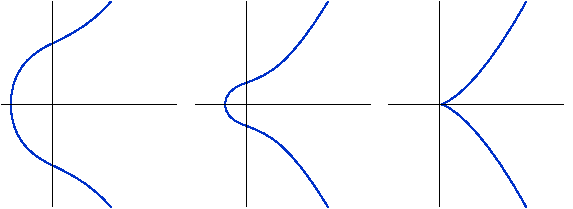
\includegraphics[scale=0.9,viewport=0 0 61 100,clip]{main/cubic-t=0,0.5,1}\quad
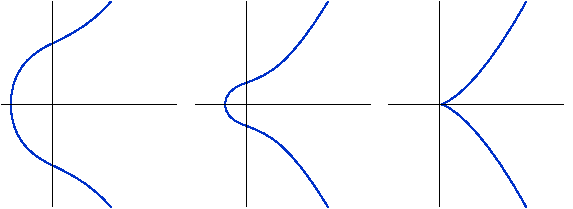
\includegraphics[scale=0.9,viewport=90 0 161 100,clip]{main/cubic-t=0,0.5,1}\quad
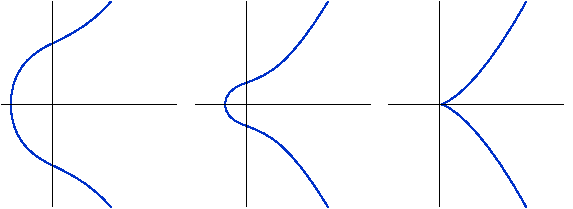
\includegraphics[scale=0.9,viewport=190 0 261 100,clip]{main/cubic-t=0,0.5,1}
\centerline{\hfil
\footnotesize
\hbox to 1.2in{\hfil\hfil$t=1$\hfil}\enspace
\hbox to 1.2in{\hfil\hfil$t=0.5$\hfil}\enspace
\hbox to 1.2in{\hfil\hfil$t=0$\hfil}\hfil
}
\caption{A curve of genus 1 degenerating to a cuspidal curve in the family $
C_t = V(y^2 -x^3 - t^2x - t^3)$.
}
\index{cuspidal curve!of genus 1}%
\label{smooth to cusp}
\label{Fig7.A}
\end{figure}

When modular compactifications do exist, they are extremely valuable
for the study of both the space $M$ and of the objects parametrized
by $M$: compactness allows us to apply the techniques of modern
algebraic geometry to the space $\ovM$, while the fact that
it is still a moduli space gives us a handle on its \null geometry.
In the following section, we will describe a modular compactification
of $M_g$. The objects parametrized are called \textit{stable curves}.

Getting back to the moduli space $\ovM_1$, if we have a family where
$j(\lambda)$ has a pole, we would like to say that the limit of the curves in the family is an irreducible nodal curve,
but this is not necessarily true! For example, the limit of the curves
$$
y^2 = x(x-t)(tx-1)
$$
as $t \to 0$ is reducible, with two components meeting in two points, 0 and $\infty$.
What is true is that a process called
\emph{semistable reduction}
\index{semistable reduction}%
shows that after a base change and a birational
modification of the family around the pole we can replace the family with one where the singular fiber
is indeed an irreducible nodal curve
(Figure~\ref{unstable to stable}).
See \cite{MR1631825} for a description of this process in
general, and several explicit examples.

\begin{figure}
\centerline{\includegraphics[width=2in,height=3in]{"main/Fig07-1"}\llap{\hskip-0.5in
\footnotesize\openup-2pt
\raise100pt\vbox{\hbox{blow down a}\hbox{component}\hbox{of central fiber}}}}
\caption{In this case a birational modification of the
total space of the family changes the unstable reducible curve to a stable curve.}
\label{unstable to stable}
\end{figure}

\section{Higher genus}

The  idea  is  analogous to the one used  for genus 1 curves: to
construct a moduli space, first parametrize curves with a choice of
some additional structure, such as a map to projective space, and then
mod out by the choices made. For any smooth projective curve $C$ of
genus $g\geq 2$, the tricanonical linear series
\index{tricanonical linear series}%
\index{linear series!tricanonical}%
$|3K_C|$ is very
ample; it embeds $C$ as a curve of degree $6g-6$ in $\PP^{5g-6}$. Thus
we have a way of realizing a given abstract curve $C$ as a curve in
projective space, unique up to automorphisms of $\PP^{5g-6}$.

We claim next that the set of smooth, tricanonically embedded curves
is a locally closed subset $X$ of the
Hilbert scheme
\index{Hilbert scheme}%
$\Hilb_{(6g-6)m+1-g}(\PP^{5g-6})$ parametrizing curves of genus $g$
and degree $6g-6$ in $\PP^{5g-6}$. By Lemma~\ref{smooth is open}, the
set of points in the base over which the curves are smooth is open. Let
$$
\Hilb^\circ = \Hilb^\circ_{(6g-6)m+1-g}(\PP^{5g-6})\subset \Hilb_{(6g-6)m+1-g}(\PP^{5g-6})
$$
be this open set.

Next, on the universal family
$\cC \subset \Hilb^\circ \times \PP^{5g-6}$,
we have two families of invertible sheaves: we have the
pullback of $\cO_{\PP^{5g-6}}(1)$; and we have the cube $K^3$ of the
dualizing sheaf. Each gives rise to a section of the relative
Picard variety
\index{Picard variety}%
over $\Hilb^\circ` `$, and the locus where they agree is thus a
closed subset $X \subset \Hilb^\circ` `$.

The group $\PGL_{5g-5}$
of automorphisms of $\PP^{5g-6}$ acts on the variety $X$ and its orbits
\index{PGL@$\PGL_{5g-5}$}%
are the isomorphism classes of smooth curves of genus $g$; thus, we might hope to realize the moduli space $M_g$ as the quotient of $X$ by $\PGL_{5g-5}$. But here things go awry in a hurry: unlike the case of an action of a finite group on a variety,
the orbit spaces of infinite groups are often not algebraic varieties.
(Think of the action of $\CC^*$ on $\CC$ by multiplication.) What is
needed is a tool to extract the ``best possible approximation'' to a
quotient. Happily, David Mumford created a tool that does exactly this:
\emph{geometric invariant theory}
\index{geometric invariant theory}%
\index{Mumford, David}%
(GIT).  To see how GIT can be
used in this  setting to produce the space $M_g$, see the wonderful
introduction in \cite{Mumford-Suominen}
or the more technical version in \cite{MR0450272}.

\begin{theorem}[Mumford]\label{unproved1}
The space of orbits of $\PGL_{5g-5}$ acting on the subset of the Hilbert scheme representing
tricanonical curves has the structure of an algebraic variety $M_g$ which is a \emph{coarse moduli
space} in the
\index{coarse moduli space}%
following
sense:
\begin{enumerate}
 \item Given any flat family $Y\to B$ of smooth curves of genus $g$ there is a morphism of schemes
$B\to M_g$ sending each closed point $p\in B$ to the point of $M_g$
representing the fiber $Y\!_b$.
 \item These maps form a natural transformation from the functor $G(-)$ of families of smooth curves to the functor $\Mor_{\mathrm{ schemes}}(-,@ M_g)$
through which any natural transformation $G \to \Mor_{\mathrm{ schemes}}(-,@ M')$
 factors.
\end{enumerate}
\end{theorem}

The power of the theory of the moduli space of curves was greatly increased when compactifications of the space (there are many interesting ones) were introduced. One of these, the compactification
\index{modular compactification}%
of $M_1 = \AA^1$ to $\ovM_1 = \PP^1$ by adding a nodal curve, has already been mentioned. This has the desirable properties that the subset added to $M_1$ is a divisor; and the compactification is \emph{modular} in the sense
that the point added corresponds to a curve almost of the same type as the curves in $M_1$.

There are two reasons why a compactification is  important:
\index{compactification}%
\index{compactification|seealso{modular}}%

First, the great majority of the techniques that algebraic geometers
have developed for dealing with varieties apply directly only to
projective varieties. For example, the
Satake compactification
\index{Satake compactification}%
is a projective variety containing $M_g$ in such a way that the
complement\emdash usually referred to as the
boundary\emdash has
codimension 2. Taking successive hyperplane sections that pass through
a given point but don't meet the boundary, we see that for $g\geq 2$
there is a complete one-dimensional family of \emph{smooth} curves
containing any smooth curve of genus $\geq 2$.

Often, though, we can learn the most from a compactification where the
added boundary
is a divisor, and this is the case for the Deligne--Mumford compactification
\index{Deligne--Mumford compactification}%
$\ovM_g$, described below,  introduced
in the
groundbreaking 1969 paper \cite{Deligne-Mumford}.
A central example of how this is used is given in
Section~\ref{mgunirational}, where we take up the question, ``can we
write down a general curve of genus $g$?''

To describe this compactification, we first explain some of the language and results of geometric
invariant theory.

\subsection*{Stable, semistable, unstable}

Given a quasiprojective variety $X \subset \PP^N$ and a group $G \subset \PGL_{N+1}$ that carries $X$ into itself, we wish to construct as good a map as possible from the set of orbits
to a projective space. Whatever map we take, the closure of the
image will correspond to a graded ring. We want to preserve as much of the structure of the orbit space as possible, and on an open affine cover
this means finding as many functions as possible that are invariant on
the orbits. Thus it is natural to take the
ring of invariants
\index{invariant!ring of --s}%
\index{ring of invariants}%
of the homogeneous coordinate ring $A$ of the closure of $X$ as the homogeneous coordinate ring of the closure
of the image of $X$.

The first difficulty is that the elements of $A$ are not functions on $X$, so $G$ may not even act on $A$. However,
it is possible to lift the action of $G$ to an action on $A$ of the
slightly larger group, $\SL_{N+1}$, a process called
\index{linearization}%
\emph{linearization}. The kernel of the map $\SL_{N+1} \to \PGL_{N+1}$
consists of diagonal matrices of finite order dividing $N+1$, and the choice of
a linearization amounts to a choice of a character of this abelian
group. However, the choice doesn't
matter,
since the kernel acts trivially on forms of degree a multiple
of $N+1$,
and thus
the action of $\PGL_{N+1}$ itself  extends to an action on the
homogeneous coordinate ring of the $(N+1)$-st Veronese embedding.
Another way to say this is to introduce the cone $\overkern31 X
\subset \AA^{N+1}$ over $X$; a linearization amounts to an action of
$\SL_{N+1}$ on $\overkern31 X$.%
{\meshing\par}

The second difficulty in this program is that the ring of invariants
of an infinite group may not
be finitely generated,
so it may not correspond to a projective variety. Hilbert showed that if $G= \SL_{N+1}$, then the ring of invariants
is finitely generated. Since Hilbert's time this result has been extended to the class of
\emph{linearly reductive}
\index{linearly reductive group}%
groups\emdash see \cite{MR0382294}.
Thus the subring $A^G \subset A$ of invariant elements is finitely generated over the ground field.

The third difficulty is that the points of $\Proj(A^G)$, usually
\index{'/'@$\quot$|defi}%
denoted $X\quot G$, are generally not in one-to-one correspondence
with the orbits of $G$ on $X$!

Geometric invariant theory explains the relationship of $X\quot G$ to the set of orbits. To do this, it performs a sort of triage on the points of $X$ (or their orbits), dividing them into three classes: stable, semistable and unstable. The theory also provides tools for determining this stratification.


\begin{enumerate}
\item  \emph{Stable points}. These are the points whose orbits in
\index{stable point|defi}%
$\AA^{N+1}$ are closed. They comprise an open subset
$X^{\mathrm{stable}} \subset X$, and the points of an open subset of
$X\quot G$ correspond one-to-one to the stable orbits, that is, an open subset
\index{set-theoretic equality}%
that is
set-theoretically
$X^{\mathrm{stable}}/G$. In general, this
set may be empty, but in the case of the action of
$\PGL_3$
on the
\index{PGL@$\PGL_3$}%
$\PP^9$ of
plane cubics,
\index{plane cubic}%
the stable points are the smooth plane
cubics, and the quotient is the affine $j$-line.

\index{stable point|defi}%
\item \emph{Strictly semistable points}.
\index{semistable point|defi}%
\index{strictly semistable point|defi}%
These are the points $p$ such that there exists an invariant form not
vanishing at $p$.  Together with the stable points, comprise a larger
open subset $X^{\mathrm{{semistable}}} \subset X$, called the
\emph{semistable} locus. Two  semistable points $p,q$ map to the same
point in $X\quot G$ if and only~if $\overkern20{Gp}\cap
\overkern20{Gq}\cap X^{\mathrm{{semistable}}} \neq \emptyset$. In the
example of the action of $\PGL_3$ on  $\PP^9` `$, the semistable
locus contains  the orbits of smooth and nodal plane cubics; that is,
smooth cubics together with the three orbits consisting of irreducible
cubics with a node, unions of lines and conics meeting transversely,
and triangles. In the quotient, these last three orbits correspond to
just one additional point, and this quotient is the
compactification of the affine line
\index{compactification!of the affine line}%
to the projective line obtained by adding one point.

\item  \emph{Unstable orbits}. These are the
\index{unstable points|defi}%
points $p$ on which all invariant polynomials vanish, so that the induced map
$\Proj A \to \Proj (A^G)$ is not even defined at $p$. Thus unstable
points do not correspond to any points of $X\quot G$; in fact, they
cannot be included in any topologically separated quotient of an open
subset of $X$ defined in this way, though there may be other
compactifications, coming from
other representations of $M_g$ as $X'\quot  G'$; see \cite{MR3044128}.
\end{enumerate}

\section{Stable curves}

The compactification $\ovM_g$ is also a
\emph{modular} compactification
\index{modular compactification}%
\index{compactification!modular}%
in the sense that the points of the boundary correspond to slightly more
\index{stable curve}%
general objects of the same type as the points of $M_g$.

\begin{definition}
A reduced irreducible connected curve is \emph{stable}
\index{stable curve|defi}%
if it has at most nodes as singularities and if every smooth rational
component meets the other components at least three times
(Figure~\ref{complicated stable curve}).

\begin{figure}[b]
\centerline {\includegraphics[height=1.2in]{"main/Fig07-2"}}
\caption{A stable curve.}
\label{complicated stable curve}
\end{figure}

The last phrase of the definition could be replaced by the equivalent condition that the automorphism group
of $C$ is finite.
\end{definition}

These are stable points in the Hilbert scheme of tricanonical
embeddings in the sense of geometric invariant theory, and the result
is that $M_g$ has a modular compactification that is a
projective variety:

\begin{theorem}[properties of $\ovM_g$
\cite{Deligne-Mumford,MR702954}]%
\hskip-20pt % first item shouldn't run inline because the headline is full
\label{DM is coarse}%
\begin{enumerate}
 \item $\ovM_g$ is a projective variety.
 \item The points of $\ovM_g$ correspond one-to-one to isomorphism classes of smooth curves.
 \item For every family $\cC \to B$ of stable curves there is a morphism of schemes $B\to M_g$ carrying
 each closed point  $b \in B$ to the point representing the isomorphism class of the fiber of $\cC$ over $b$.
 These maps form a natural transformation from the functor $G(-)$ of families of stable curves to the functor
$$\Mor_{\mathrm{ schemes}}(-,@ \ovM_g)$$
through which any natural transformation $G \to \Mor_{\mathrm{ schemes}}(-,@ M')$
 factors.
\end{enumerate}
\end{theorem}

The deepest theorems about $M_{g}$ have been proven using the
divisor class group
\index{divisor class group}%
 of $\ovM_{g}$,
and many of the divisors that play a role are actually supported on
the complement $\ovM_{g} \setminus M_{g}$, often called the
\emph{boundary}.
\index{boundary|defi}%
{\meshing\par}

\begin{fact}
\it
For $g\geq 1$ the boundary $\ovM_{g}\setminus M_{g}$ is the
union of $@1+\lfloor{g/2}\rfloor$ divisors whose generic points are
\begin{enumerate}
 \item irreducible nodal curves of geometric genus $g-1$
and
 \item for $@i = 1, \dots,\lfloor{g/2}\rfloor$
the union of two smooth curves $C_{i}\cup C_{g-i}$ of genera
 $i$ and $g-i$ meeting in a point.
\end{enumerate}
\vskip-1.4\baselineskip
\end{fact}

We will not prove either of Theorems~\ref{unproved1}
and~\ref{DM is coarse}. For an introduction to the
proofs, with references, see \cite{MR1631825}.

\subsection*{How we deal with the fact that $\ovM_g$ is not fine}

The fact that $\ovM_g$ is not a fine moduli space\emdash and that
correspondingly
there does not exist a universal family
\index{universal family!nonexistence}%
of curves over
it\emdash is unquestionably a nuisance. Nonetheless, there are ways of
dealing with the situation. The first step is to identify the cause of
the problem, which is that some curves have nontrivial automorphisms.
There are three ways to proceed:
\index{automorphism}%

\begin{enumerate}
\item \emph{Kill the automorphisms}. The idea here is to add
additional structure to the objects parametrized, so as to eliminate
automorphisms. Here is an example of such a construction. We saw in
Chapter~\ref{JacobianChapter} that on a smooth projective curve $C$
of genus $g$, the collection of invertible sheaves $\cL$ with $\cL^m
\cong \cO_C$ forms a group isomorphic to $(\ZZ/m)^{2g}$. We define a
\emph{curve with level $m$ structure}
\index{curve!with level $m$ structure|defi}%
to be such a curve, together with a choice of $2g$ generators
$\cL_1,\dots,\cL_{2g}$ for this group. On every curve $C$ of genus
$\geq 2$ an automorphism fixing all line bundles of order $m \geq 3$
is trivial, and there does
exist a fine moduli space $M_g[m]$
\index{M@$M_g[m]$}%
for curves with level $m$ structure; this space is a finite cover of
$M_g$. Thus, while a universal family does not exist over $M_g$, one
does exist over a finite cover of $M_g$, and this is sufficient for
many purposes.

\item \emph {Ignore the automorphisms}.
Here we use a basic fact, which we'll establish in Section~\ref{curves with automorphisms}: in $M_g$, the locus $A \subset M_g$ of curves that do have automorphisms other than the identity has codimension $g-2$. If we restrict to the complement $M_g^\circ = M_g \setminus A$, accordingly, there does exist a universal family, and again this is sufficient for many purposes; for example, if $g \geq 4$ then a divisor class on $M_g$ is determined by its restriction to $M_g^\circ$, so we can just work over that open set.

\item \emph{Embrace the automorphisms}. We mentioned above that there
  does not exist a fine moduli space for curves of genus $g$ in the
  category of schemes. But there is a larger category, called
\emph{stacks},
\index{stack}%
in which a fine moduli space does exist. This solution to the problem, pioneered by Deligne and Mumford, has
many advantages but involves a substantial investment in mastering the technical issues; readers who wish to pursue this avenue may consult \cite{Deligne-Mumford}, \cite{Olsson}, or the forthcoming book {\it Stacks and moduli} by Jarod Alper.
\index{Alper, Jarod}%
\end{enumerate}


\section{Can one write down a general curve of genus $g$?}\label{mgunirational}

We have made a fuss over the value of compactifying $M_g$ to a projective variety. To see an example of the usefulness of $\ovM_g$, we'll take up a question we've raised before: Can one write down a general curve of genus $g$?
More precisely,  does there exist a family of curves depending freely
on parameters that includes all the curves in an open subset of
$M_{g}$,
as the equation $y^{2} = x(x-1)(x-\lambda)$
represents general curves of genus 1? Still more precisely,
we say that a variety is \emph{unirational}
\index{unirational|defi}%
if it admits a
dominant morphism
\index{dominant map}%
from an open subset of $\AA^{n}$.
Our question is: Is $M_g$ unirational?

We have produced  families with free parameters in genera 2 and 3. Essentially
the same approach works in genera $4$ and $5$; in each case a general
canonical curve is a
complete intersection,
\index{complete intersection}%
so that if we take the coefficients of its defining polynomials to be
general scalars we have a general curve.

This method breaks down when we get to genus 6, where a canonical curve is not a complete intersection. But it's close enough: as discussed in Chapter~\ref{Brill--Noether}, a general canonical curve of genus 6 is the intersection of a smooth del Pezzo surface $S \subset \PP^5$ with a quadric hypersurface $Q$; since all smooth del Pezzo surfaces in $\PP^5$ are isomorphic, we can just fix one such surface $S$ and let $Q$ be a general quadric.

It gets harder as the genus increases. Already genus 7 calls for a
different approach. Here we want to argue that, by
Brill--Noether theory,
\index{Brill--Noether theory}%
a general curve of genus $7$ can be realized as (the normalization of)
a plane
septic curve
\index{septic curve}%
with 8 nodes $p_1,\dots,p_8 \in \PP^2` `$. Conversely, if $p_1,\dots,p_8 \in \PP^2$ are general points then having nodes at the points $p_i$ imposes $ 3\times 8 = 24$ independent conditions on the $\PP^{35}$ of curves of degree 7, so that we would expect that the septic curves double at the $p_i$ form a linear series, parametrized by a projective space $\PP^{11}$.

This suggests that we consider the space
$$
\Sigma \colonequals \bigl\{@ (p_1,\dots,p_8,C) \in (\PP^2)^8 \times \PP^{35} 
\mid C \text{ is singular at } p_1,\dots,p_8 @\bigr\}
$$
With a little work, we can see that there is a unique component $\Sigma^\circ$ of $\Sigma$ dominating $(\PP^2)^8` `$, which is a $\PP^{11}$-bundle over an open subset of $(\PP^2)^8$ and hence rational; this component dominates $M_7$, showing that $M_7$ is unirational.

A similar approach works through genus 10, and Severi conjectured that
\index{Severi, Francesco}%
it would be possible to do something similar for all genera. The
approach through plane curves, however, fails in genus 11: by the
Brill--Noether theorem,
\index{Brill--Noether theorem}%
the smallest degree of a planar embedding of a general curve of genus
11 is 10; by Theorem~\ref{grd omnibus} (itself a consequence of
the Brill--Noether theorem), such a curve has $\tbinom{9}{2}-11 = 25$
nodes. But $3 \times 25 > 65$, the dimension of the space of plane
curves of degree 10. Thus, if we introduce the analogue of the
incidence correspondence
\index{incidence correspondence}%
we used in the case of genus 7\emdash that is,
$$
\Sigma \colonequals\bigl\{@(p_1,\dots,p_{25},C)\in(\PP^2)^{25} \times \PP^{65} 
\mid C \text{ is singular at } p_1,\dots,p_{25} @\bigr\}
$$
\emdash
then the projection $\Sigma \to (\PP^2)^{25}$ is not dominant, and we have no idea if $\Sigma$ is rational.
Ad hoc (and much more difficult) arguments have been given in genera
11, 12, 13 and 14, but so far no-one can go further in producing
general curves; in genus 15 it is only known that
 any two general curves can be 
\null connected by a chain of rational curves that passes through
the locus of irreducible nodal curves in $\ovM_{g}$
\cite{MR2202246}. In genera 15 and 16 Chang and Ran showed
the  weaker statement
that $\ovM_{g}$ has no pluricanonical divisors.%
\looseness=-1
{\meshing\par}

However the issue is resolved for all genera $\geq 22$. Surprisingly, this depends (in the current state of our knowledge) on an understanding of the complement
$\ovM_{g}\setminus M_{g}$ and its image in the divisor class group of
$\ovM_{g}$. The starting point is the fact that a smooth
$n$-dimensional projective variety $X$ with an effective
pluricanonical canonical divisor\emdash that is, a nonzero section of
the sheaf $\omega_{X}^{\otimes p}$ for some $p>0$\emdash cannot be
unirational: if there were a
dominant rational map
\index{dominant map}%
$\PP^n \to X$, we
could pull this section back to get an effective pluricanonical
divisor on $\PP^n` `$, which doesn't exist because
the canonical divisor on $\PP^{n}$ has negative degree. At the same
time, we can analyze the divisor class theory of the space $\ovM_g$
and for large $g$ exhibit an effective pluricanonical divisor on $M_g$
by using components of  $\ovM_{g}\setminus M_{g}$.
The upshot is this:

\begin{npt}
\begin{theorem}[\cite{Harris-MumfordModuli,HarrisModuli,Eisenbud-HarrisModuli,M22-23}]
For all $g \geq 22$, $M_g$ is not unirational.
\unif
\end{theorem}
\end{npt}

In each case, what is actually proven is the stronger but more
technical statement that $\ovM_g$ has \emph{general type}.
\index{general type}%
This line of argument requires a great deal of work; the interested reader
can find more details, plus a guide to the literature, in
\cite{MR1631825}.

\section{Hurwitz spaces}\label{Hurwitz spaces}

Hurwitz spaces are spaces parametrizing branched covers. They are fascinating objects; we know quite a bit about their geometry but there is much that is unknown as well. In this discussion, we'll stick to the simplest case, that of the \emph{small Hurwitz spaces}, parametrizing simply branched covers of $\PP^1` `$.
\index{Hurwitz space|(}%
\index{simply branched cover}%

To start with the definition: the small Hurwitz space $\Hur^\circ_{g,d}$
\index{Hur@$\Hur^\circ_{g,d}$|defi}%
parametrizes pairs $(C, f)$ where $C$ is a smooth
curve of genus $g$ and $f : C \to \PP^1$ a map of degree $d$ with
simple branching; that is,
$$
\Hur^\circ_{g,d} = \bigl\{@(C, f) \mid C \in M_g
\text{ and } f:C \to \PP^1 \text{ simply branched of degree } d@\bigr\}.
$$

There are two natural maps from the Hurwitz space to other spaces.
First, we can ``project on the first factor;'' that is, simply forget
the map $f$ to arrive at a map $\pi : \Hur^\circ_{g,d} \to M_g$.
Secondly, we can associate to a point $(C,f) \in \Hur^\circ_{g,d}$ the
branch divisor $B \subset \PP^1` `$, which is an unordered $b$-tuple
of distinct points in $\PP^1` `$, which we can think of as a point in
the $b$-th symmetric product $(\PP^1)_b  \cong \PP^b` `$. We thus have
a diagram
\vspace*{-10pt} % meshing
$$
\small
\xymatrix@C=15pt@R=25pt{
 & \Hur^\circ_{g,d} \ar[ld]_\pi  \ar[rd]^\beta & \\
M_g  & & U \subset \smash{\PP^b}
}
\index{beta@$\beta$ (Hurwicz spaces)}%
$$
where $U \subset \PP^b$ is the complement of the hypersurface in $\PP^{b}$ where at least 2 of the
$b$ points are equal, called the
discriminant hypersurface.
\index{discriminant hypersurface|defi}%
Thus the Hurwitz space is positioned between an object $U$ we
understand relatively well, and an object $M_g$ about which we would
like to know more; this accounts for the historical importance of
Hurwitz spaces. We'll now illustrate how this can be exploited.

To begin with, by the analysis in Section~\ref{branched covers}, we
see that \emph{the map $\beta$ is a covering space}: for any reduced
divisor $B \subset \PP^1$ there are a finite number of simply branched
covers of $\PP^1$ with branch divisor $B$; and as we vary the points
of $B$ locally we can deform the cover along with them. This allows us
to give the Hurwitz space $\Hur^\circ_{g,d}$ the structure of a smooth
variety, and also tells us that
$$
\vspace*{-4pt}
\dim(\Hur^\circ_{g,d}) = b = 2d+2g-2.
\vspace*{-4pt}
$$

\subsection*{The dimension of $M_g$}

Next, we look at the projection $\pi : \Hur^\circ_{g,d} \to M_g$. To
\index{M0g@$M_g$!dimension}%
start, let's assume $d$ is large relative to $g$; $d \geq g+1$
suffices, but you can take $d$ as large as you like; taking $d > 2g$
may make the argument simpler.

\begin{proposition}
If $d \geq g+1$, the map $\pi :
\Hur^\circ_{g,d} \to M_g$ is surjective, with fibers of dimension $2d-g+1$.
\end{proposition}

\begin{proof}
The question is, how many simply branched maps $f : C \to \PP^1$ of
degree $d$ are there
for a given curve $C$?
To begin with, the
$g+1$ theorem
\index{g plus 1@$g+1$ theorem}%
(Theorem \ref{g+1 theorem}) tells us that
there are some, whence we see that $\pi$ is surjective.

We can compute the dimension of the fibers, too.
\kern-1pt To specify a map
$f {:}@ C {\to} \PP^1`$,
we can start by choosing a divisor $D \in C_d$, which
will be the divisor $f^{-1}(\infty)$; this can be a general divisor of
degree $d$ on $C$. Second, we choose a divisor $E$ which will be
$f^{-1}(0)$; this can be a general member of the linear system $|D|$,
which has dimension $d-g$. Finally, specifying $f^{-1}(\infty)$ and
$f^{-1}(0)$ determines the map $f$ up to scalar multiplication on
$\PP^1$; adding up the degrees of freedom, we see that the fibers of
$\pi$ have dimension
$$
d + (d-g) + 1 = 2d-g+1.
\qed
$$
\let\qed\relax
\end{proof}

Finally, we conclude that if $g\geq2$ then
$$
\dim(M_g) = (2d+2g-2) - (2d - g + 1) = 3g-3.
$$

We can use this in turn to analyze the cases of smaller $d$. As a
basic application, note that the group $\PGL_2$ of automorphisms of
$\PP^1$ acts on the Hurwitz space: given $\varphi \in \PGL_2$, we can
send $(C,f)$ to $(C, \varphi \circ f)$. Moreover, the orbits of this
action lie in fibers of the projection $\pi : \Hur^\circ_{g,d} \to M_g$,
meaning that the fibers of $\pi$ have dimension at least 3.

\begin{corollary}\label{branched cover BN}
If $d < \bigl\lceil \frac{g}{2} \bigr\rceil + 1$, then a general curve
$C$ of genus $g$ does not admit a map of degree $d$ to $\PP^1` `$.
\unif
\end{corollary}

This is one-half of the case $r=1$ of the
Brill--Noether theorem,
\index{Brill--Noether theorem}%
about which we will say much more later.

\subsection*{Irreducibility of $M_g$}

Another important application is the original proof of the
\index{Hurwitz, Adolf}%
\index{M0g|$M_g$!irreducibility}%
irreducibility of $M_g$. Hurwitz \citeyear{Hurwitz} analyzed the
\index{monodromy}%
\index{historical context}%
monodromy of the map $\beta: \Hur^\circ_{g,d} \to U \subset\PP^b$,
which describes what happens
when you let the branch
points of a cover wander around in $U$ before coming back to their
original locations. He proved that the monodromy is transitive, and
hence that the Hurwitz space $\Hur^\circ_{g,d}$ is irreducible; since
$\Hur^\circ_{g,d}$ dominates $M_g$ for $d$ large, he deduced that $M_g$
must be irreducible as well.

Hurwitz's argument illustrates a fundamental point: in practice,
moduli spaces of curves ``with extra structure,'' such as a map to
projective space, are often easier to work with, and provide a useful
tool for understanding the geometry of abstract moduli spaces. Given an abstract curve $C$ of genus $g$, it's
hard without developing a fair amount of deformation
theory, to show that $C$ varies in a nontrivial family. But if
$C$ is expressed as a branched cover, we can find such families just
by varying the branch points.

There are many open problems connected with the Hurwitz scheme; here are a few:
\begin{enumerate}
\item A compactification of the Hurwitz scheme by
\index{admissible cover}%
\emph{admissible covers}
(allowing both source and target
of the covering to be reducible in a controlled way) is known \cite{MR1631825}, but the boundary is very complicated, and it would be interesting to find a simpler one.

\item It is conjectured that the
Picard group
\index{Picard group}%
of the Hurwitz scheme is torsion; see \cite{MR3320849},
where the conjecture is proved
for $g\leq 5$, and \cite{mullane} for the case $d>g-1$.

\item There is active work and many open problems around computing the
\emph{Hurwitz numbers},
\index{Hurwitz number|defi}%
that is,
the number of curves having maps to $\PP^{1}$ with specified degree and branching; see for example \cite{Hurwitz2} and \cite{ELSV}.
\index{Hurwitz space|)}%
\end{enumerate}

\section{The Severi variety}\label{severi variety}

Despite having been studied for so long, many questions about plane
curves remain open\emdash for example: which ones degenerate into
which others, and in what way. All plane curves of degree $d$ have the
same Hilbert function, and thus the same
arithmetic genus
\index{arithmetic genus}%
$\tbinom{d-1}{2}$, but since curves of degree $d$ can have different
sorts and numbers of singularities, they can have geometric genera
from 0 to $\tbinom{d-1}{2}$. In this section we will explore the
subset of (reduced, irreducible) curves of degree $d$ with a fixed
\index{geometric genus}%
geometric genus. We will focus on the open set consisting of
nodal curves (those with only nodes as singularities),
and compute its dimension.

\def\Vdg{V_{\mskip-6mu d,g}}
\def\Vdgbar{\overkern1{17}{\Vdg}}
\def\Vdgpbar{\overkern1{19}{V_{\smash{\!d,g'`}}}}

Let $\PP^N \colonequals  \PP^{\sbinom{d+2}{ 2} - 1}$ be the projective space parametrizing plane curves of degree $d$.
Within $\PP^N$ the set of reduced irreducible curves is open\emdash it is the complement of the union of the images of the maps
$$
\PP^{\sbinom{d_1+2}{ 2} - 1}\times\PP^{\sbinom{d_2+2}{ 2}-1} \to \PP^N
$$
with $d_1+d_2 = d$ given by multiplication of forms.

\begin{definition}
The \emph{Severi variety}
\index{Severi variety|defi}%
$\Vdg \subset \Vdgbar$ is the locus of irreducible plane curves of
\index{V0gd@$\Vdg$|defi}%
degree $d$ with $\delta = \tbinom{d-1}{2} - g$ nodes and no other
singularities. This is a locally closed subset of $\PP^N` `$.
(Reason: having only nodes as singularities is an open condition; having at least a certain number of them
is a closed condition.)
It is sometimes
\index{small Severi variety|defi}%
called the \emph{small Severi variety}, since we are excluding curves with more complicated singularities.
\end{definition}

We will see that the closure $\Vdgbar$ is well behaved in a
neighborhood of $\Vdg$; but away from this, even the singularities
of $\Vdgbar$ are not well understood. It
is an interesting open
problem to find a simpler partial compactification of $ \Vdg$.

\begin{fact}\label{severi irreducible}
Corollary~\ref{local geometry of Severi} says that
the variety $\Vdg$ is smooth. In 1921 F. Severi gave an incorrect
proof
that $\Vdg$ is
connected, and thus irreducible.
\index{Severi, Francesco}%
\index{historical context}%
A~correct proof was finally given in \cite{MR837522}.
\end{fact}


\subsection*{Local geometry of the Severi variety}

We first consider the
\index{universal singular point}%
\index{Severi variety!local geometry}%
universal singular point
$$
\Phi \colonequals  \left\{ (C, p) \in \PP^N \times \PP^2 \mid p \in C_{\sing} \right\}
$$
and its image $\Delta\subset \PP^N` `$, the \emph{discriminant variety}.
\index{discriminant variety}%

\begin{proposition}
\label{local severi geometry}
 $\Phi$
is smooth and irreducible of dimension $N-1$,
and the discriminant $\Delta$ is a hypersurface in $\PP^N` `$.
\unif
\end{proposition}

\begin{proof}
Projection on the second factor expresses $\Phi$ as a $\PP^{N-3}$-bundle over $\PP^2` `$. Explicitly, if $[X,Y,Z]$ are homogeneous coordinates on $\PP^2` `$, and $\{a_{i,j,k} \mid i+j+k = d \}$ are homogeneous coordinates on $\PP^N` `$, then the universal curve
$$
\CC \colonequals  \left\{ (C, p) \in \PP^N \times \PP^2 \mid p \in C \right\}
$$
is given as the zero locus of the single bihomogeneous polynomial
$$
F([a_{i,j,k}], [X,Y,Z] ) = \sum a_{i,j,k} X^iY^jZ^k
$$
of bidegree $(1, d)$;
and the universal singular point is the common zero locus of the three partial derivatives $\partial F/\partial X$, $\partial F/\partial Y$ and  $\partial F/\partial Z$.

The set of forms $F$ that define curves singular at a given point is
defined by~3 independent linear conditions, and since the set of
points is 2-dimensional,
the set $\Delta$ of singular forms has dimension $N-1$.
\end{proof}

We next compute the differential of the map $\pi : \Phi \to \PP^N$:

\begin{lemma}\label{tangent space to discriminant}
Suppose that $(C,p)\in \Phi$, with $p$ a node of $C$.  The differential
$$
d\pi : T_{(C,p)}\Phi \to T_C \PP^N
$$
is injective, with image the hyperplane $H_p \subset \PP^N$ of plane curves containing the point $p$.
\end{lemma}

Thus, if $p$ is a node of $C$ and the only singularity of $C$, then $\Delta$ is smooth at $C$; and more generally the image of a small analytic neighborhood of $(C,p) \in \Phi$ is smooth, and we can identify its tangent space at $p$ with the hyperplane $H_p$.

\begin{proof}
We will prove this using affine coordinates on $\PP^2$ and $\PP^N` `$.
Changing coordinates if necessary, we may assume that the point
$[1,0,0]$ is not in $C$, and that the point $p$ is $[0,0,1]$.
Let $x = X/Z$ and $y = Y/Z$ be coordinates on the affine plane $Z \neq 0$ and
write the polynomial $F(x,y,1)$ above as
$$
f(x,y) = \sum_{i+j \leq d} a_{i,j} x^iy^j
,
$$
with $a_{d,0}$ normalized to 1.

Let $g,h$ be the two partial derivatives of $f$:
\begin{align*}
 g(x,y) \colonequals  \frac{\partial f}{\partial x} &= \sum_{i+j \leq d} i a_{i,j} x^{i-1}y^j\\
h(x,y) \colonequals  \frac{\partial f}{\partial y} &= \sum_{i+j \leq d} j a_{i,j} ix^{i}y^{j-1}.
\end{align*}
The functions $f, g$ and $h$ are local defining equations for $\Phi$;
we consider their partial derivatives with respect to $x, y$ and
$a_{0,0}$, evaluated at the point $(C,p)$, as in
the table:
$$
     \begin{array}{lccc} % <-- Alignments: 1st column left, 2nd middle and 3rd right, with vertical lines in between
            & f & g & h \\
      \hline
\vbox to 11pt{} %strut
\unfrac{\partial}{\partial x} & 0 & a_{2,0} & a_{1,1} \\
\unfrac{\partial}{\partial y} & 0 & a_{1,1} & a_{0,2} \\
\unfrac{\partial}{\partial a_{0,0}} & 1 & 0 & 0
    \end{array}
$$

The fact that $p$ is a node of $C$ (and not a more complicated singularity) implies that the upper right $2 \times 2$ submatrix is nonsingular, which shows that the differential $d\pi$ is injective, and its image is the hyperplane $a_{0,0} = 0$ in $\PP^N` `$, which is exactly the hyperplane of curves containing $p$.
\end{proof}

\begin{lemma}\label{adjoint independent}
The nodes $q_i$ of an irreducible nodal plane curve $C$ of degree $d$
\index{node!condition imposed by}%
\index{independent conditions}%
impose independent conditions on curves of degree $d-3$, and hence on
curves of any degree $m \geq d-3$.
\end{lemma}

\begin{proof}
We will prove in Chapter~\ref{PlaneCurvesChapter} that the $g$ sections of the canonical sheaf on the normalization $\widetilde C$ of
$C$ are the preimages of the sections of $\sO_C(d-3)$ that vanish at the nodes. On the other hand,
$h^0(\sO_C(d-3)) = \tbinom{d-1}{2}$, and the difference is exactly the number of nodes.
\end{proof}

\begin{corollary}\label{local geometry of Severi}
\hskip-1.6pt
If $C$ is a nodal curve of degree $d$
and
geometric genus
$g =\nobreak \tbinom{`d-1` `}{2}-\nobreak\delta$, then in a neighborhood of $C\in \PP^N$
the discriminant hypersurface of all singular curves consists of $\delta$ smooth sheets, meeting transversely, and hence
$\Vdg$ is smooth.

In a neighborhood
of
 $C \in \PP^N$
the variety
$\Vdgpbar$
with $g' =  \tbinom{d-1}{2}-\delta' >g$
is the union of $\tbinom{\delta}{\delta'\!}$ smooth branches, each of
dimension $N - \delta'$, corresponding bijectively with subsets of
$\{p_1,\dots,p_{\delta}\}$ of cardinality $\delta'$.
\meshing
\end{corollary}

Figure~\ref{Severi discriminant} shows the case $\delta=2$,  $\delta' = 1$.
\begin{figure}[b]\label{discriminant of a Severi locus}
\centerline {\includegraphics[height=1.6in]{"main/Fig07-3"}}
\vskip-8pt
 \caption{%
Near
the point corresponding to a plane curve with 2 nodes,
$V_{d,@\protect\sbinom{d-1}{2}-2}$ is the
transverse
intersection of two smooth hypersurfaces.}
 \label{Severi discriminant}
\end{figure}


\begin{proof}
Lemma~\ref{tangent space to discriminant} shows that in an analytic neighborhood of $C\in \PP^N$ the discriminant hypersurface $\Delta$  consists of $\delta$ smooth sheets, each corresponding to one node, and Lemma~\ref{adjoint independent} implies that the tangent spaces to these sheets are linearly independent.
\end{proof}

\begin{corollary}\label{dim Severi}
The  Severi variety $\Vdg$ has pure dimension $N - \delta$, where
$$\delta = \tbinom{d-1}{2} - g.$$
\end{corollary}

In Section~\ref{estimating dim hilb}, we give a heuristic calculation
\index{expected dimension}%
\index{h@$h(g,r,d)$|defi}%
of the ``expected dimension'' $h(g,r,d)$ of the variety parametrizing
curves of degree $d$ and genus $g$ in $\PP^r$:
$$
h(g,r,d) \colonequals  4g-3 + (r+1)(d-g+1) - 1.
$$
The actual dimension of the restricted Hilbert scheme may be quite different. But  Corollary~\ref{dim Severi} shows that in case $r=2$ (as in the case of $r=1$), the actual dimension is always the expected.



\section{Exercises}

\begin{exercise}
Consider the action of $G_m$ on $\PP^3$ given in coordinates by
$$t: (x_0,x_1,x_2,x_3) \mapsto (tx_0,\ tx_1,\ t^{-1}x_2,\ t^{-1}x_3)
$$
for $t\in G_m = \CC^*` `$.
\begin{enumerate}
 \item Show that the ring  of forms in $\CC[x_0, \dots, x_3]$ that are
invariant
\index{invariant form}%
is generated by
$$
x_0x_3, \ x_0x_2,\ x_1x_3,\ x_1x_2
$$
and thus $\PP^3\quot @G_m\cong \PP^1\times \PP^1` `$.
\item Show that the
unstable locus
\index{unstable locus}%
for this action is the union of the two lines $x_0=x_1=0$ and
$x_2=x_3=0$.
\item Show that the orbits of $G_m$ are the points on the unstable lines and, for each
point $p$ not on an unstable line, a copy of
$\PP^1\setminus \{0,\infty\}\cong G_m$ whose closure is the unique line containing $p$ and
meeting both unstable lines.
\end{enumerate}
\end{exercise}

\begin{exercise}
Consider the action of $G_m$ on $\PP^3$ given in coordinates by
$$t: (x_0,x_1,x_2,x_3) \mapsto (tx_0,\ tx_1,\ tx_2,\ t^{-1}x_3)
$$
for $t\in G_m = \CC^*` `$.
\begin{enumerate}
 \item Show that the ring  of forms in $\CC[x_0, \dots, x_3]$ that are invariant is generated by
 forms
\index{invariant form}%
$$
F(x_0,  x_1, x_2)x_3
$$
where $F$ is a cubic form on $\PP^2` `$, and thus
$\PP^3\quot@G_m\cong \PP^2` `$, with the embedding given by the
third Veronese map.
\index{Veronese!map!third}%
\item Show that the unstable locus for this action is the union of the point  $x_0=x_1=x_2 = 0$ and
\index{unstable locus}%
the plane $x_3=0$.
\item Show that the orbits of $G_m$ are the points on the components of the unstable locus and, for each
point $p$ that is not unstable, a copy of
$\PP^1\setminus \{0,\infty\}\cong G_m$ whose closure is the unique line containing $p$ and the unstable
point. Thus the quotient map is the composition of the linear projection from the unstable point with the 3-uple
embedding.
\end{enumerate}
\end{exercise}

\begin{exercise}\label{not fine 1}
Show from the explicit formula for the
\index{j@$j$-function}%
$j$-function
on page~\pageref{formula for j}
that if $j : B \to M_1 = \AA^1$ is a
map  associated to a family $\cC \to B$ of curves of genus 1, then
every zero of the $j$-function has multiplicity divisible by 3, and
conclude that some maps $B\to M_1$ do not correspond to families of
curves; in particular there is no universal family over $M_1$, and
thus $M_1$ is not a fine moduli space for curves
of genus 1. There is a similar problem at $j(\lambda)=1728$.
\end{exercise}

\begin{exercise}\label{not fine 2}
In Exercise~\ref{not fine 1} we saw a local obstruction to the
\index{universal family!nonexistence over $M_1$}%
existence of a universal family over $M_1$. There is also a global
obstruction, coming from the fact that some genus 1 curves have extra
automorphisms. Show that there is a ``tautological'' family over the
punctured $j$-line $L \colonequals  \AA^1\setminus \{0,1728\}$\emdash
that is, a family
$\sX \to L$ whose fiber over $t$ has $j$-invariant $t$; but show that this family is not universal as follows:

Let $B$ be any curve of genus 1 and $\tau : B \to B$ a translation of
order 2, and let $E$ be a fixed
elliptic curve
\index{elliptic curve}%
(that is, a curve of
genus 1 with a chosen point, so that we may identify the points of $E$
with an abelian group).
Let $\cX\to L$ be the family $E\times B$ modulo the equivalence
relation $(e,b) \sim (-e, \tau(b))$.
The projection to $B/\tau$ has all fibers isomorphic to $E/(\pm) \cong E$. But the family is not
isomorphic to the trivial family $E\times B/\tau \to B/\tau$.
\tohint{8-04}
\end{exercise}

